Searching a unordered database in a classical computer is of \(O(N)\) complexity, where N is the number of entries, simply iterating through every item in the database and questioning the oracle; however in 1996 Lov Grover discovered a method of searching a database in \(O(\sqrt{N})\) complexity. The problem of searching a database is defined by finding the entry with the least amount of computational cost. Grover's algorithm is based on the fact that in a quantum computer it is possible to parallelise many queries to the oracle in a single step. This is very different compared to a classical algorithm which would require the oracle to be queried once for every item, hence the \(O(N)\) complexity. Grover went further than just discovering a search algorithm: he proved that it is impossible to accomplish this task in less time.

Grover's Algorithm consists of three main stages and results in a quantum register very likely to be the resulting answer we are looking for. These stages are:

\begin{enumerate}
 \item Initialisation
 \item Grover Iteration
	\begin{itemize}
		\item Oracle (\(U_w\)) 
		\item Diffusion Operator (\(U_s\)) 
	\end{itemize}
 \item Measurement
\end{enumerate}

The first stage, initialisation, sets the quantum register that will be acted upon into a complete superposition of all basis states. This is done by applying a Hadamard operator to each qubit within the quantum register. The resulting quantum register of this stage is \cite{lomo2000}:

\begin{equation}
 \ket{\psi} = \frac{1}{\sqrt{N}} \sum_{i=0}^{N-1} \ket{i}
\end{equation}

The second stage of Grover's Algorithm is the most complex of the three and involves mathematics that will not be covered \cite{lomo2000}, however final results will be given. During this stage an Oracle functioning in a way such that it can identify the answer (\(x_0\)) is required. The Oracle is a black box function which is represented by \cite{lomo2000}:

\begin{equation}
 f(x) = \left\{
	\begin{array}{lr}
		1 & if \: x = x_0 \\
		0 & otherwise
	\end{array}
	\right.
\end{equation}

The Oracle is a unitary transform of the quantum register it acts upon. The basis that represents the answer is phase shifted by \(\pi\), while the other bases are unchanged. Note that the phase shift does not have a classical analogue.

After the Oracle, another transform is applied: the Diffusion operator. This is defined by \cite{lomo2000}:

\begin{equation}
 U_s = -HI_{\ket{0}}H
\end{equation}

The Diffusion operator is unitary and is equivalent to an inversion about the mean values of the amplitudes of each state. In effect it increases the amplitude of \(\ket{x_0}\) and decreases the amplitude of the other bases.

By applying both the Oracle and the Diffusion operator a number of times to the resulting quantum register from the previous stage, the amplitude of the answer base increases. A representation of this process is a rotation of the quantum register in a two dimensional complex space from the initial superposition vector towards the \(\ket{x_0}\) basis. The number of steps required can be calculated by \cite{lomo2000}:

\begin{equation}
 k = \left \lfloor\frac{\pi}{4}\sqrt{N} \right \rfloor
\end{equation}

During the final stage of the algorithm, the resulting quantum register from the Grover iteration is measured, which causes it to collapsed into a specfic basis. This measurement results in a single base state with a non-zero amplitude and all other states with zero amplitudes, hence measuring again will always result in the same measurement. The probability that the answer state is obtained by the measurement is \cite{lomo2000}:

\begin{equation}
 Prob(\ket{x_0}) \geq 1 - \frac{1}{N}
\end{equation}

To test whether the correct result was retrieved the oracle can be queried to recognise the measurement, if it does not recognize it as the answer, the algorithm is restarted from the beginning.

Below is a graphical representation of the change of probabilities during the application of Grover's Algorithm.

If we assume the required answer (marked state) is 4 with 8 different possible states. 

\begin{figure}[H]
	\centering
	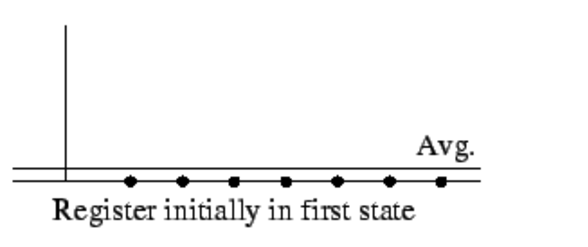
\includegraphics[width=70mm]{./images/grover_initial}
	\caption{The quantum register is initially prepared in the first state where base 0 has an amplitude of 1 and the rest have a zero amplitude. \cite{grovergraph} }
\end{figure}

\begin{figure}[H]
	\centering
	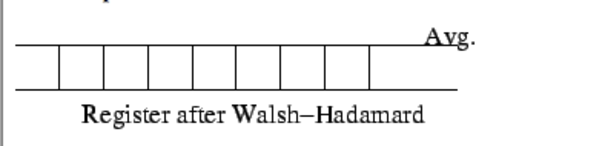
\includegraphics[width=70mm]{./images/grover_hadamard}
	\caption{A Hadamard gate is then applied which puts the QRegister into an equal superposition of all possible states. \cite{grovergraph}  }
\end{figure}

\begin{figure}[H]
	\centering
	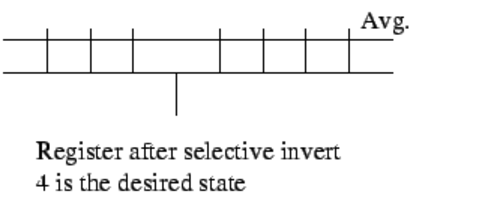
\includegraphics[width=70mm]{./images/grover_invert}
	\caption{When the Oracle is applied it goes through selective phase inversion. This switches the sign of the amplitude of the marked state. \cite{grovergraph} }
\end{figure}

\begin{figure}[H]
	\centering
	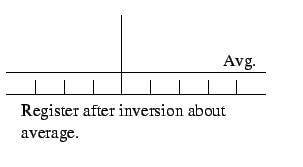
\includegraphics[width=70mm]{./images/afterinv}
	\caption{The Diffusion matrix then performs an inversion about average operation. This increases the amplitude of the state inverted in the previous step. \cite{grovergraph} }
\end{figure}
